\chapter{INTRODUCTION}
\label{chap:introduction}

Mobile computing is the preferred method of personal computing for
millions of users.
%
The mobile device market has grown over 400 million smartphones shipped
in 2011 and an estimated prediction of 1 billion shipments for
2015~\cite{market}.
%
This growth has been inspired by the hundreds of thousands of mobile
applications such as social networking, location-based services, image
processing, augmented reality, face and speech recognition.
%
To meet the increasing demands of these computationally-intense
applications, mobile platforms have been augmented with multi-core CPUs,
more powerful GPUs and other specialized hardware accelerators.
%
Despite of these many enhancements to the mobile platform's hardware,
however, the inescapable fact is that their limited batteries will
always serve as a bottleneck while hindering the mobile platforms from
utilizing their computing capabilities.\\
%
%To address this restriction, there have been research efforts on remote
%offloading systems which seek intelligent ways to enable mobile platform
%developers to leverage computing capabilities of more powerful
%resources over the network.
%
%Even though existing approaches provide core mechanisms to transform
%typical mobile applications to offloading-enabled applications through
%various granulaities of prtitioning and migration, they still lack
%considerations for a service discovery mechanism while assuming the
%vavailability of remote computing nodes with static endpoints.
%
%Moreover, they have not investigated data privacy and secure
%communcation between the mobile client and remote resources, which can
%be a crucial flaw for the mobile computing environment.\\
%
To address this issue, there have been research efforts in two different
areas: 1) heterogeneous computing and 2) cloud offloading.
%
Heterogeneous computing has been seen as a  mechanism to increase the
dynamic range of execution by combining computing elements of varying
power performance characteristics and opportunistically scheduling the
workloads onto the optimal computing element based on the workload
requirements and energy availability~\cite{chen}.
%
Heterogeneous architectures with big/small cores, CPU/GPU and
CPU/Hardware accelerators are now being offered by leading processor/SoC
vendors~\cite{bigprocessing, tegra}.
%
By allowing dynamic scheduling of workload onto the best processing
element based on the requirements, these architectures provide a wide
dynamic range of execution providing performance when needed and
optimizing for energy performance.\\
%
In addition, computation offloading has been proposed as an alternative
for extending the capabilities of mobile platforms.
%
Computation offloading in a mobile environment is more constrained than
previously studied cyber-foraging~\cite{cyber} techniques in traditional
computing systems, because mobile networks have less throughput, and can
exhibit higher latencies and variances.
%
In the past few years, there have been various mobile offloading
techniques proposed in the context of constrained mobile environments,
from application partitioning~\cite{maui} or process
migration~\cite{hung} to full mobile environment
cloning~\cite{clonecloud}.\\
%
This proposal presents a novel framework which enables remote workload
offloading to external resources within a mobile user's \lq\lq Social Area
Network\rq\rq\ in which trusted remote computing resources such as family or
friend's ones are involved regardless of user mobility.
%
The proposed system accomplishes this by 1) utilizing a peer-to-peer
virtual private networking technique as a substrate for the discovery
and configuration of trusted remote resources, and 2) extending OpenCL
framework, which is an open standard of parallel programming for
heterogeneous computing environment, to support remote offloading using
the TCP/IP networking stack.
%
OpenCL is a framework specifically designed to offload workloads in
heterogeneous platforms, but it currently does not support access to
accelerators across the network.
%
Although the proposed offloading system is not the first to present the
concept of offloading heterogeneous workloads over the
network(i.e.Remote CUDA~\cite{rcuda}, Virual OpenCL~\cite{vopencl}), but
it is the first to consider the approach where offloading happens
between a mobile device and remote resources such as a workstation or a
virtual machine instance running in the cloud.\\
%
The prototype implementation of the proposed framework is evaluated,
with regard to end-to-end application performance and energy
consumption in mobile devices, through a variety of network
configurations representing local and wide area network, and various
levels of remote computing capabilities such as typical CPUs, GPUs as
well as Amazon EC2 instances.
%
According to the evaluation, the proposed architecture achieves more
energy efficient performance by offloading than executing locally
depending on the characteristics of mobile workloads and network
conditions.\\
%
Based on the evaluation results, mobile workloads are characterized for
the suitability of offloading from the perspective of computation to
communication ratio which is a comprehensive measurement mirroring
network conditions and workload requirements.
%
In addition, this dissertation proposes applying machine learning
techniques to a runtime scheduler for mobile offloading framework.
%
By adopting machine learning techniques to the remote offloading
scheduling problem, a scheduler can be automatically trained from
previous offloading behaviors and make decisions on whether mobile
workloads should be offloaded or executed locally according to past
behaviors and current conditions.
%
While running various machine learning algorithms, the evaluation shows the
feasibility of adopting machine learning techniques into the scheduler
problem for mobile offloading framework.
%
\section{Related Works on Remote Offloading Systems for Mobile Platforms}
\label{intro:relatedwork}

The research community has been investigating different methods to
offload computation for decades.
%
However, remote execution to the cloud has created new opportunities to
explore novel offloading solutions.
%
This section discusses the most recent proposals for mobile computation
offloading which fall in the following categories: application
partitioning, thread or application migration, and distributed
offloading frameworks.
%
\subsection{Application Partitioning}
\label{intro:app_partitioning}
%
This approach involves selecting portions of an application to execute
remotely through the use of a static or dynamic scheduler.
%
In Spectra~\cite{spectra}, developers identify functions in the
application that  can be offloaded to a remote server over RPC.
%
By monitoring the CPU, file system, and bandwidth, Spectra dynamically
decides at runtime which portions of the application should run locally
or remotely.
%
MAUI~\cite{maui} takes a similar approach but alleviates the process by
using many of programming features in the.NET platform such as method
attributes, and the Reflection API.
%
Through the .NET Framework's virtual machine, MAUI is able to
dynamcially serialize and ship \textit{remotable} methods and data to a
server proxy, thus leveraging the server's superior processing
capabilities while saving power on the mobile device.
%
Cuckoo~\cite{cuckoo} takes a slightly modified approach by focusing more
on integrating with the Eclipse IDE.
%
However, it requires developers to implement both local and remote
versions of their functionality, whereas MAUI only requires annotations
instead of a different implementation.
%
At runtime, Cuckoo does intelligent offloading by determining the
appropriate cases to run the code locally or remotely.
%
The proposed approach may be classified as application partitioning
similar to Cuckoo because developers does not have to worry about the
complications of shipping the workload to the remote device.
%
\subsection{Thread Migration}
\label{intro:thr_migration}
%
The source code modification required for most partitioning schemes can
preclude adoption by many applications.
On the other hand, thread and process migration can be achieved without
any source code modification.
%
CloneCloud~\cite{clonecloud} achieves this by  employing thread
migration in the Dalvik Java Virtual Machine(JVM) by transferring all of
the thread state(thread stack, necessary heap objects and registers) to
the remote virtual machine.
%
When the remote thread completes, the results are merged back with the
local Dalvik JVM memory stack.
%
The authors of COMET~\cite{comet} developed a similar thread migration
technique by doing application VM synchronization through a distributed
shared memory(DSM) model.
%
The proposed solution does not require any thread stack or heap
synchronization because the OpenCL framework requires explicit
declaration of input and output buffers for remote kernel execution.
%
Hence, the use of OpenCL alleviates the complexities of memory
synchronizaitons since all of the necessary state is encapsulated as
contiguous memory array that are managed through a few OpenCL data
offloading fucntions(i.e. \textit{clEnqueueReadBeffer},
\textit{clEnqueueWriteBuffer}, \textit{clEnqueueMapBuffer}).
%
\subsection{Application Migration}
\label{intro:app_migration}
%
The previous thread migration techniques can be technically challenging
to implement since they require memory synchronization between the
remote thread and other threads running locally.
%
All local threads have to block on dirty region of the heap that has
been offloaded to the remote server until the remote execution finishes
and the memory is merged and released.
%
Application migration does not have such requirements.
%
Hung et al.~\cite{hung} describes an application migration design that
leverages the \textit{onResume} and\textit{onPause} events of an Android
application as the markers for process migration.
%
The \textit{onPause} event occurs when a user switches to another
application.
%
The Android system requires that application states are saved on
persistent storage in the case the operating system decides to shutdown
in the case of low memory situations.
%
Hence, Hung et al. create a solution which uses the \textit{onPause}
event to force the application to save its state.
%
The state is then copied to a cloned VM running on the cloud and resumed
there until completion, then transferred back.
%
The proposed design automatically handles the state transfers between
the local and remote devices without relying on specific Android-based
events.
%
\subsection{Distributed Offloading Framework}
\label{intro:framework}
%
Various recent approaches have focused on a totally different model
requiring more effort from the developers.
%
Proposals such as Mobile Map Reduce(MMR)~\cite{mobileMR},
Sonora~\cite{sonora}, Serendipity~\cite{serendipity}, and
ThinkAir~\cite{thinkair} expose a distributed offloading framework for
developers to adopt.
%
For example, MMR is a MapReduce system optimized for the constrained
networking conditions of mobile devices byu taking into account
bandwidth and latency for efficient mobile device performance.
%
Sonora exposes a distributed stream-based programming model which
handles workload distribution and failures in a mobile network.
%
Serendipity provides an offloading framework for intermittently
connected mobile ddevices and does not rely on cloud services.\\
%
The proposed approach can be also classified as a distributed offloading
framework.
%
Instead of defining the system from scratch, however, the proposed
framework reuses the workload offloading paradigms of the OpenCL
framework which provides a more familiar and widely supported interface
for developers.
%
There also exist other heterogeneous offloading frameworks which are
quite similar to the proposed approach.
%
Remote CUDA~\cite{rcuda} is one approach that extends the NVIDIA CUDA
API to support remote offloading over the network.
%
Their goal is to minimize the network overhead and they analyze the
impact of using different networking technologies such as Gigabit
Ethernet or InfiniBand.
%
Their research is aimed at cluster environment such as the data center
and it does not consider mobile environments with low bandwidth.
%
Virtual OpenCL\cite{vopencl} provides a similar solution which uses
OpenCL instead of the proprietary CUDA protocol.
%
They also focus on cluster environments but they leverage the MPI
library for memory and workload synchronization.
%
Since our solution is designed for mobile platforms and the cloud, it
differs greatly because it takes into account not only performanc, but
also energy consumption, connectivity, and mobility.
%
\subsection{Lack of Privacy and Trust}
\label{intro:lack}
%
Mobile devices tend to process more private information about their
users.
%
Hence, dealing with trust and privacy is a fundamental requirement.
%
None of these previous works thoroughly deal with the issue of securing
the offloaded data in a trusted fashion.
%
They also do not address the issue of verifying the integrity of the
results provided by the remote cloud server.
%
Hung et. al mentioned using L2TP VPN for security, but such as approach
does not ensure privacy within the cloud which is a growing concern for
many cloud applications~\cite{brodkin}.
%
Private communication and tursted results are amongst the first issues
that this proposal addresses through the use of a peer-to-peer virtual
private network(P2PVPN). 
%
The proposed approach guarantees that the user data is only offloaded to
trusted compute nodes and verified through non-repudiable, encrypted
channels.
%
I also analyze the cost associated with providing this privacy because
encryption on a mobile device is non-negligible.
%
However, none of previous approaches measured this cost.
%
UIA~\cite{uia} has considered ad-hoc virtual private networks connecting
mobile devices of social peers, and is closely related to SocialVPN, but
has not been evaluated in the context of computation offloading.\\
%
Apart from the above mentioned offload solutions, there has been a lot
of research work going on in the area of heterogeneity which deals with
combining processing elements of varying power performance capabilities
to the local processor/platform.
%
A combination of small and big cores, GPUs and special purpose hardware
optimally scheduled for best energy efficient performance based on
workload requirement and better power provides a wider dynamic execution
range.
%
\section{Motivation}
\label{intro:motivation}
This section describes a few scnarios that motivate the proposed
approach in detail.
%
Figure~\ref{fig:motivation} gives a eneral idea of one example deployment scenario.
%
Alice connects her smartphone to a virtual private network(VPN)
consisting of her laptop, Bob's desktop, and her virtual machine
instance running on Amazon EC2.
%
Since each of these devices is running SocialVPN~\cite{socialvpn}, they
automatically join the same virtual private network creating a pool of
trusted resources in a Social Area Network.
%
With this secure IP layer consisting of trusted peers, the framework is
able to use IP multicasting over the VPN to discovery nodes that are
available for computation offloading.
%
During the discovery process, the system records the characteristics of
each node in the network such as bandwidth, latency, and processing
capabilities.
%
When an application decides to offload some computation, the framework
dynamically determines the best node to use as the remote offloading
target.
%
In many cases, for example, if the bandwidth or remote processing
capabilities are too low, the framework may decide to simply run the
workload locally.\\
%
The goal of the design is to provide an intuitive offloading framework
that developers can integrate into their application using well-adopted
programming concepts.
%
Currently, many software developers utilize the OpenCL framework to
exploit on-board heterogeneous platforms.
%
In the scientific computing arena, supercomputers increasingly integrate
CPUs and GPus in order to maximize performance/Watt~\cite{powertutor}.
%
Popular software projects, such as OpenCV and OpenSSL, are
re-implementing major portions of their functions to run on the OpenCL
platform.
%
Mobile SoC platforms, based on processors such as ARM and Intel, are
also starting to provide OpenCL support on their architecture.
%
The latest version of the OpenCL specification allows for devices
beyond CPUs and GPUs to be accesses through the API.
%
There is also an industry momentum building up behind OpenCL with the
formation of new industry foundations to foster fast
adoption~\cite{gregor}.
%
These considerations point to OpenCL API as the emerging defacto
standard for heterogeneous computing.\\
%
\begin{figure}
\centering
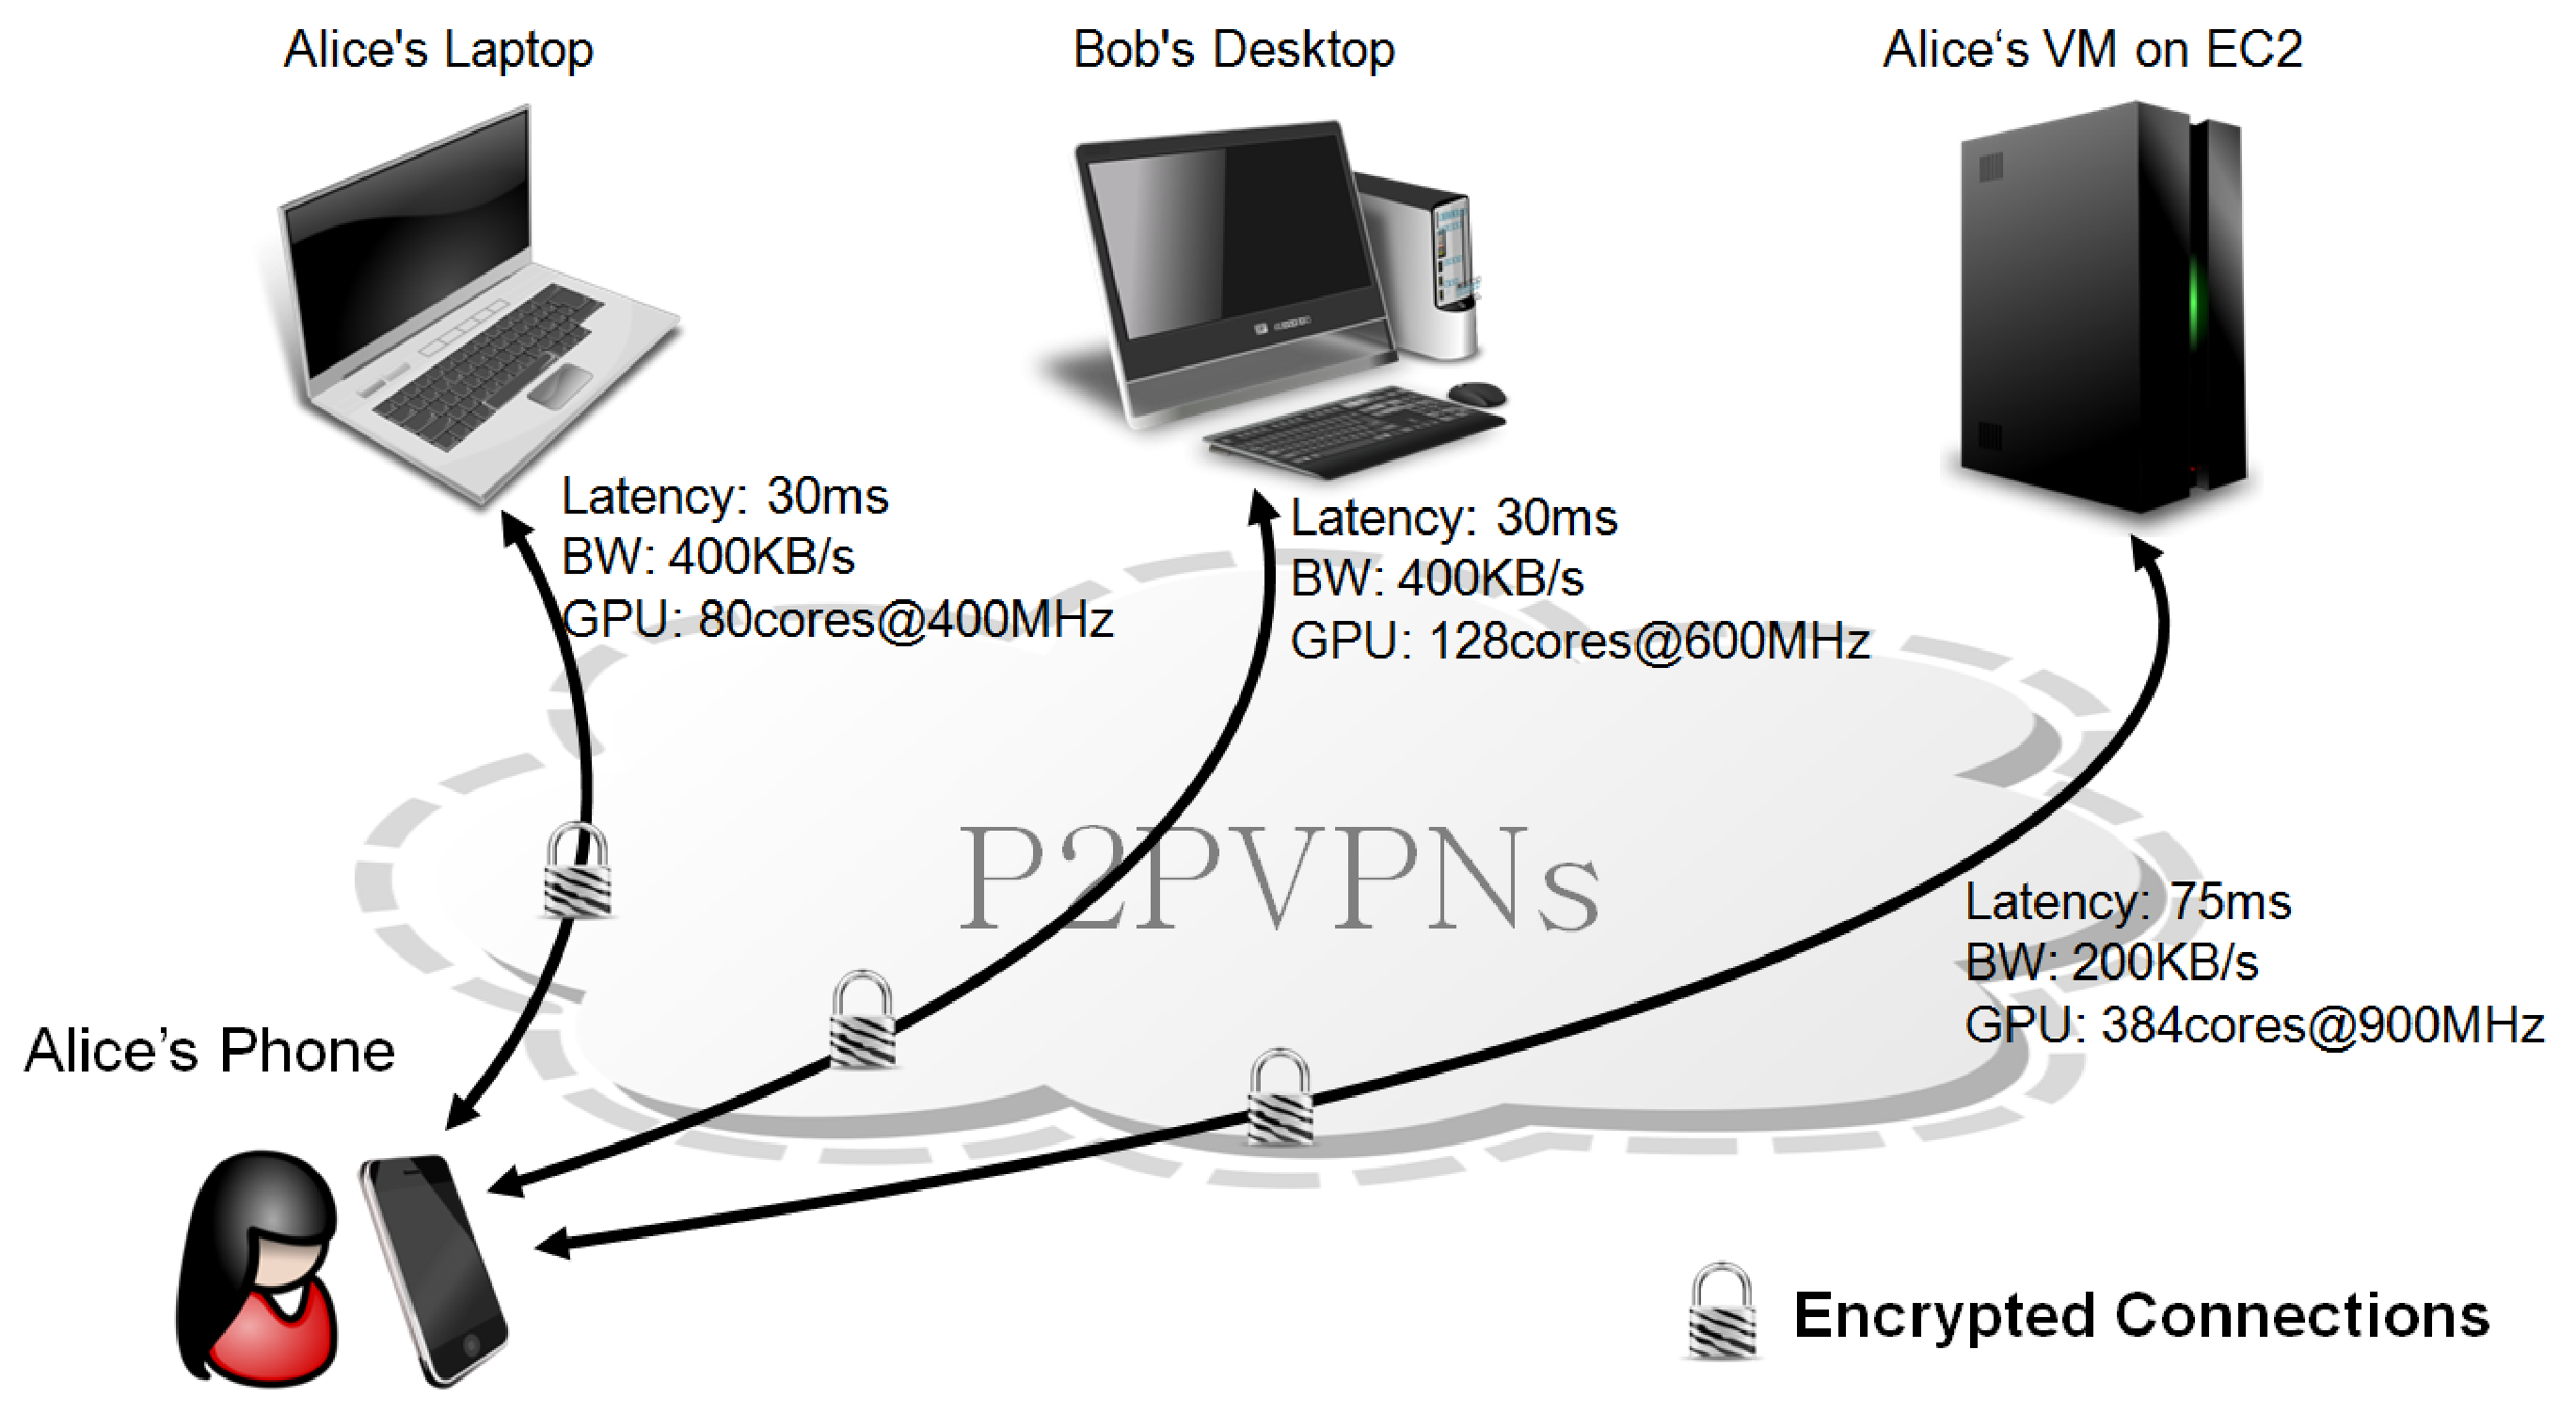
\epsfig{file=figs/motivation.eps, width=5.5in}
\caption{Private Networking and Node Selection}
\label{fig:motivation}
\end{figure}
%
Here is another example of how a developer might take advantage of
OpenCL and the proposed platform in a seamless fashion.
%
Consider a typical facial recognition application in a mobile device
used as a security feature, or for tagging friends on a social
networking application.
%
First, the developer utilizes a CPU implementation.
%
However, the developer quickly realizes the processing limitations of
doing image processing on the CPU and decides that such a workload is
better suited for the GPU or another hardware-based accelerator.
%
With this realization, the developer writes an OpenCL-based
implementation due to its wide support and adoption.
%
Using OpenCL, the developer is able to offload the computation from the
mobile CPU to the mobile GPU and therefore achieve better performance
with less battery consumption.\\
%
The proposed framework aims to extend the umbrella of heterogeneous
computing to include devices beyond the physical host platform.
%
By recompiling the application to link with the proposed framework, the
developer can transparently access remote resources available via the
SocialVPN, including GPUs running on computing resources more powerful
than a mobile device.
%
For instance, if the mobile device is connected to a virtual network
consisting of an Amazon EC2 GPU instance, and the user's personal
workstation, the extensions to the OpenCL framework will automaticallu
select the best candidate based on available device capabilities, and
network conditions as the target compute node for remote execution.
%
Also, the use of SocialVPN, ensures that computation is offloaded
securely to socially trusted nodes.
%
This enhancement occurs transparently to the developer and the user
requiring only code recompilation. 
%

\section{Contributions}
\label{intro:contributions}
The key contributions of this dissertation can be summarized as
follows:\\
%
{\bf Novel framework for remote computation offloading.} The primary
contribution is a novel framework which addresses the challenge of
remote computation offloading to resources in the cloud the paradigm of
extended hardware-layer heterogeneous computing.
%
Heterogeneous computing uses specialized hardware accelerators to
increase computing throughput and performance.
%
The proposed framework combines the power of cloud offloading with the
flexibility of heterogeneous architecture which expands the dynamic
execution range of mobile platforms, which are typically restricted by
power constraints.\\
%
{\bf Decentralized resource discovery mechanism.} Second
contribution of this proposal is a distributed method of resource
management which handles service discovery, access control, and data
privacy.
%
Previous mobile offloading solutions have not investigated a service
discovery mechanism by assuming the availability of remote conputing
resources with static endpoints.
%
The proposed framework advocates a dynamic approach where candidate
computing nodes are discovered at runtime while allowing for a more
flexible design.
%
By using IP multicast-based discovery, the proposed system periodically
locates computing nodes which are available within their social area
network.\\
%
{\bf Machine learning-based runtime scheduler.} Prior studies have
primarily focused on core mechanisms for offloading.
%
However, adaptive scheduling in such system is important because
offloading effectiveness can be influenced by varying network
conditions, workload requirements, and load at the target device.
%
In this dissertation, a study on the feasibility of applying machine
learning techniques to address the adaptive scheduling problem in mobile
offloading framework is presented as a third contribution.
%
By taking the algorithm complexity and scheduling performance into
account, a few machine learning algorithms are selected to implement
on/offline runtime schedulers for mobile offloading framework.\\
%
The prototype implementation of the proposed framework is evaluated,
with regard to end-to-end application performance and energy consumption
in mobile devices, through a variety of network configurations
representing local and wide area network, and various levels of remote
computing capabilities such as typical CPUs, GPUs as well as Amazon EC2
instances.
%

\section{Future Work}
\label{intro:futurework}
The proposed remote offloading framework for mobile platforms will be
further extended into 1) the consideration of multiple remote computing
resources and the provision of the best resource in accordance with
mobile application requirements, and 2) the modularization of the
machine learning-based runtime scheduler.
%
\subsection{On-Demand Server Provision}
\label{intro:serverprovision}

To correctly implement the UF ETD \latex\  template in accordance with the UF Gradschool Editorial Office Guildlines. The following files and/or packages are required: %
\begin{enumerate} %
    \item MiKTex \vspace{-10pt}%
    \item Some text editor\vspace{-10pt}
    \item Hanging Package \vspace{-10pt}%
    \item Caption Package \vspace{-10pt}%
    \item Hyperref Package %
 \end{enumerate} %NOTE: this paragraph continues without an indent. 
 % If you put a space between the list and the next paragraph it will automatically start a new paragraph
 This is an example of a ``short�� list. Not because there's only 5 items on the list but because each item is less than one line in length. Since short lists are relatively rare the default spacing for the itemize and enumerate environments is for the ``long'' list where at least one item on the list wraps to a second line. In order to generate a correct short list you need to insert a \verb=\vspace{-10pt}= command after all but the last item on the short list. \citep{Huang92}

The enumerate and itemize environments have been modified to meet Editorial Office guidelines (A special thank you to Antonio Paiva for both the suggestion and the code) but require the ufenumerate.sty file to be in the same folder as your main file. It is loaded via the usepackage\{ufenumerate\} command. The itemize environment is modified by a set of commands in the usersetcommands file.

\subsection{Modularization of Machine Learning-based Runtime Scheduler}
\label{intro:modularization}

If you need to add a package please remember to place it before the hyperref package in the packages file. Hyperref needs to have several modifications in place to work properly and is essential for the required links. To ensure that it works correctly it must be the last package loaded - and even then it's a delicate operation.

The following programs are not needed but may be very useful when editing documents in \LaTeX:  \begin{itemize} %
    \item WinEDT: This text editor is recommended for use editing \TeX-files as it has many useful built in macros and is easy to use  %
    \item This program can be found and downloaded here: \url{http://www.winedt.com/} %
    \item The GIMP (GNU Image Manipulation Program) %
    \begin{itemize}%
        \item A freeware graphics editing program for picture editing and file conversions %\vspace{-12pt}%
        \item Comparable to Adobe Photoshop %\vspace{-12pt}%
        \item Can be downloaded here: \url{http://www.gimp.org/}%
    \end{itemize}
    \item A good reference of \LaTeX 2\ensuremath{\epsilon} commands%
    \begin{itemize}
        \item This should be included on the ETD website here: \url{http://etd.helpdesk.ufl.edu/tex.php}
    \end{itemize}
\end{itemize} %
This is an example of ``nested'' lists. In the itemize environment you can choose an alternative symbol for the ``sub-list.'' The method of specifying this symbol is \verb=\item[-]= where the optional symbol is inserted into the square brackets. Unless you are referring to an item by number, itemized lists are generally preferable to enumerated ones. The difference between itemize and enumerate environments is illustrated by repeating this list below:\citep{Hobbie03}
\begin{enumerate} %
\item WinEDT: This text editor is recommended for use editing \TeX-files as it has many useful built in macros and is easy to use  %
\item This program can be found and downloaded here: \url{http://www.winedt.com/} %
\item The GIMP (GNU Image Manipulation Program) %
\begin{enumerate}%
\item A freeware graphics editing program for picture editing and file conversions \vspace{-10pt}%
\item Comparable to Adobe Photoshop \vspace{-10pt}%
\item Can be downloaded here: \url{http://www.gimp.org/}%
\end{enumerate}
\item A good reference of \LaTeX 2\ensuremath{\epsilon} commands%
\begin{enumerate}
\item This should be included on the ETD website here: \url{http://etd.helpdesk.ufl.edu/tex.html}
\end{enumerate}
\end{enumerate} %


\section{Outline}
\label{intro:outline}
The rest of the proposal is outlined as follows.
%
Chapter 2 provides the necessary background and context for this
proposal.
%
Chapter 3 presents the key idea of extending an OpenCL standard to
support remote offloading framework.
%
The decentralized resource discovery mechanism through a peer-to-peer
virtual private network is presented in chapter 4.
%
Chapter 5 characterizes mobile workloads the perspective of computation
to communication ratio.
%
Also, chapter 6 explains machine learning techniques for a runtime
scheduler for remote offloading system.
%
Finally, the future work is detailed in chapter 7.
